\documentclass[11pt]{article}
\usepackage{fontspec}
\usepackage[margin=1in,left=1.5in,includefoot]{geometry}
\usepackage{listings}
\usepackage{color}

\definecolor{dkgreen}{rgb}{0,0.6,0}
\definecolor{gray}{rgb}{0.5,0.5,0.5}
\definecolor{mauve}{rgb}{0.58,0,0.82}
\setmainfont[Ligatures=TeX]{Linux Libertine O}
% Graphic
\usepackage{graphicx}
\usepackage{float}

% Hyperlinks
\usepackage{hyperref}

% Header and footer
\usepackage{fancyhdr}
\pagestyle{fancy}
\fancyfoot{}
\fancyhead[LE,RO]{\bfseries\thepage}
\setlength{\headheight}{15pt}

% Quotes character
\usepackage[utf8]{inputenc}

% color python code
\lstset{frame=tb,
  language=Python,
  aboveskip=3mm,
  belowskip=3mm,
  showstringspaces=false,
  columns=flexible,
  basicstyle={\small\ttfamily},
  numbers=none,
  numberstyle=\tiny\color{gray},
  keywordstyle=\color{blue},
  commentstyle=\color{dkgreen},
  stringstyle=\color{mauve},
  breaklines=true,
  breakatwhitespace=true,
  tabsize=3
}

% color links
\usepackage{color}  
\usepackage{hyperref}
\hypersetup{
    colorlinks=true, %set true if you want colored links
    linktoc=all,     %set to all if you want both sections and subsections linked
    linkcolor=black,  %choose some color if you want links to stand out
    urlcolor=blue
}

\begin{document}
\begin{titlepage}
	\begin{center}

\includegraphics[width=0.6\textwidth]{images/bordeaux.png}\\[1cm]


{\large Report}\\[0.5cm]	
	
	\line(1,0){400}\\[0.2in]
	\huge{\bfseries Deep Learning}\\
	\line(1,0){400}\\[1.5cm]
	
	\noindent	
	
	\begin{minipage}[t]{0.4\textwidth}
		\begin{flushleft} \large
    	\emph{Author:}\\%
    	Manh Tu \textsc{Vu}
		\end{flushleft}
	\end{minipage}
	\begin{minipage}[t]{0.4\textwidth}
  		\begin{flushright} \large
    		\emph{Supervisor:} \\
    		Marie\textsc{Beurton-Aimar}
  		\end{flushright}
	\end{minipage}
	
	\vfill

% Bottom of the page
{\large \today}
	\end{center}
\end{titlepage}

% Front matter
\pagenumbering{arabic}

% Table content
\tableofcontents
\thispagestyle{empty}
\clearpage

% List of figures 
%\listoffigures
%\clearpage

\section*{Abstract}
In this project, we use Deep Learning method to automatic classify images from \href{https://heobs.org}{https://heobs.org} into 4 classes, include:
\begin{description}
\item[Heritage] \hfill \\ A place of cultural, historical, or natural significance for a group or society.
\item[Beings] \hfill \\ Any form of life, such as a plant or a living creature, whether human or other animal.
\item[Scenery] \hfill \\ Any form of landscapes which show little or no human activity and are created in the pursuit of a pure, unsullied depiction of nature, also known as scenery.
\item[Other] \hfill \\ Any other type of image that doesn't represent a photograph, such as painting, illustration, any object.	
\end{description}

\section{Introduction}
\section{Preparing dataset}
\subsection{Fetch all images}
The entire image dataset described on the text file "photos.txt" line by line. Each line includes the image id and image description. 
\begin{verbatim}
	 5a36f382-dbdf-11e6-95fd-d746d863c3eb | Những người ăn xin  | vie
	 5a36f382-dbdf-11e6-95fd-d746d863c3eb | Mendiants  | fra
	 17be8122-dbe0-11e6-860c-5fea02802d0a | Chợ Cũ (3) | vie
	 17be8122-dbe0-11e6-860c-5fea02802d0a | Vieux marché (3) | fra
	 400286c8-dbe1-11e6-bb4d-ff975c68de04 | Ngân hàng Đông Dương  | vie
	 400286c8-dbe1-11e6-bb4d-ff975c68de04 | La Banque de l’Indochine  | fra
\end{verbatim}
In order to get the image dataset, we have to fetch each image one by one by join the image id with heobs cdn url \href{https://cdn.heobs.org/photo/}{https://cdn.heobs.org/photo/}. For example, with the first line in the record above, we have the following URL: 
\begin{verbatim}
 https://cdn.heobs.org/photo/5a36f382-dbdf-11e6-95fd-d746d863c3eb
\end{verbatim}
We wrote a small python script to automatic read this text file \& download images one by one.
Totally, we have 144564 images in our dataset.

\subsection{Remove duplicate images}
In the "photos.txt", some image has two languages and then, it consumes two lines. As the record above, we have six lines, but actually, a half of them was duplicated. \newline
Because of the duplicate images doesn't help deep learning anything otherwise consume more time to train. So, to reject those images, before fetching each image, we check if this image id already exists or not. \newline
After removed duplicate, we have 142459 images left.
\subsection{Remove broken images}
After downloaded \& look around all images, we found that it has a lot of broken images, which can't be displayable. So, we write a small script to filter all of those broken images automatically. \newline
Finally, we have 89850 images left in our dataset.












\section{Unsuppervised Deep Learning}
Because of when classifying images by hand, it has some special case when one image may refer to more than one class. Thus, we need machine help us to make decisions by comparing two images are the same class or not. We also want to separate images of one class into multi unknown sub-classes. So, by using Unsupervision Deep Learning, we want to let the machine to classify a set of images unlabeled into some unknown classes. \newline
After some research, we found the Unsupervised Deep Embedding for Clustering Analysis\cite{dec} paper, which propose a new method that simultaneously learns feature representations and cluster assignments using deep neural networks to classify unlabeled images. They also provide the implement code at \href{https://github.com/piiswrong/dec}{https://github.com/piiswrong/dec}

\subsection{Trying to run the implement code with MNIST dataset}
The DEC has two phases:
\begin{description}
\item[Phase 1:]  parameter initialization with a deep autoencoder
\item[Phase 2:]  parameter optimization (i.e., clustering)
\end{description}
Because they already provide pretrained autoencoder weights, so we just have to test the phase 2 of DEC.\newline
We already tried to run this implement code with the latest Caffe version (Jul 2017), but it doesn't work because this Caffe model required some deprecated parameters. However, because of the code delivery with Caffe and Docker, so, we continue to try with Docker and their Caffe version.
The docker file in the original source code has exception but fixed by the following patch:
\begin{verbatim}
 -  liblmdb-dev libboost1.54-all-dev libatlas-base-de
 +  liblmdb-dev libboost1.54-all-dev libatlas-base-dev
\end{verbatim}
We'll first try to test with mnist dataset - the simplest example provided with the source code.
\subsubsection{Failure when training with CPU}
The implement code using GPU to train. However, I don't have the machine with GPU at this time, so I tried to move the entire code from GPU to CPU. However, it seem to the caffemodel phase 1 trained with GPU, and then it notwork with CPU version
\begin{verbatim}
multi_t_loss_layer.cpp:83] Forward_cpu not implemented.
multi_t_loss_layer.cpp:89] Backward_cpu not implemented.
\end{verbatim}

\subsubsection{Run success with GPU}

After get the machine with GPU (Nvidia Quadro 4000) and installed \href{https://github.com/NVIDIA/nvidia-docker}{Nvidia Docker}. We build and deploy the source code into the Docker container.\newline
After run success, the model generated \textbf{init.caffemodel} and \textbf{net.prototxt} files.\newline
Because of both the paper and the implement code doesn't tell us how to achieve the result, so, we suppose that this code will generate a caffe model and then we have to write a caffe network deploy to make this work.

\subsubsection{Build caffe deploy network model}
We modify the net.prototxt by the following changes:\newline
\newline
\textbf{Remove the Data Layer(s) that were used for training}\newline
These four layers are no longer valid, as we will not be providing labelled data:
\begin{verbatim}
layers {
    name: "data"
    type: DATA
    top: "data"
    data_param {
        seek: '00000000'
        source: "mnist_total"
        backend: LEVELDB
        batch_size: 256
    }
    transform_param {
        scale: 1.0
    }
    include: { phase: TRAIN }
}
layers {
    name: "data"
    type: DATA
    top: "data"
    data_param {
        seek: '00000000'
        source: "mnist_total"
        backend: LEVELDB
        batch_size: 100
    }
    transform_param {
        scale: 1.0
    }
    include: { phase: TEST }
}
layers {
    name: "label"
    type: DATA
    top: "label"
    data_param {
        seek: '00000000'
        source: "train_weight"
        backend: LEVELDB
        batch_size: 256
    }
    transform_param {
        scale: 1.0
    }
    include: { phase: TRAIN }
}
layers {
    name: "label"
    type: DATA
    top: "label"
    data_param {
        seek: '00000000'
        source: "train_weight"
        backend: LEVELDB
        batch_size: 100
    }
    transform_param {
        scale: 1.0
    }
    include: { phase: TEST }
}
\end{verbatim}
\textbf{Remove any layer that is dependent upon data labels}\newline
The MULTI\_T\_LOSS Layer and the SILENCE Layer are still expecting labels, but there are none to provide, thus these layers are no longer needed as well:
\begin{verbatim}
layers {
  name: "loss"
  type: MULTI_T_LOSS
  bottom: "output"
  bottom: "label"
  blobs_lr: 1.
  blobs_lr: 0.
  blobs_lr: 0.
  top: "loss"
  top: "std"
  top: "ind"
  top: "proba"
  multi_t_loss_param {
    num_center: 10
    alpha: 1
    lambda: 2
    beta: 1
    bandwidth: 0.1
    weight_filler {
      type: 'gaussian'
      std: 0.5
    }
  }
}
layers {
  name: "silence"
  type: SILENCE
  bottom: "label"
  bottom: "ind"
  bottom: "proba"
}

\end{verbatim}
\textbf{Set the Network up to accept data}\newline
The MNist data is of size 28x28 and in gray. For simplicity we will keep the batch size at 1. This new data entry point in our network looks like this:
\begin{verbatim}
input: "data"
input_dim: 1
input_dim: 1
input_dim: 28
input_dim: 28
\end{verbatim}

\subsubsection{Acquire and analytics the test result}

After run this network model with the \textbf{init.caffemodel}, we acquire the result describe as the following table:
\begin{table}[H]
\begin{center}
\begin{tabular}{| c | c | c | c | c | c | c | c | c | c | c |}
\hline
  &Predict 0 & 1 & 2 & 3 & 4 & 5 & 6 & 7 & 8 & 9 \\ 
\hline
Actual 0 & 0 & 357 & 1012 & 0 & 1900 & 24 & 95 & 705 & 3 & 35 \\
\hline
1 & 399 & 0 & 471 & 10 & 10 & 428 & 227 & 0 & 127 & 3011\\
\hline
2 & 348 & 237 & 11 & 785 & 643 & 302 & 707 & 18 & 684 & 441\\
\hline
3 & 0 & 106 & 169 & 2834 & 88 & 616 & 20 & 33 & 151 & 333\\
\hline
4 & 497 & 4 & 55 & 94 & 8 & 35 & 634 & 451 & 15 & 2278\\
\hline
5 & 3 & 20 & 2002 & 3 & 41 & 587 & 417 & 423 & 2 & 21\\
\hline
6 & 2 & 1083 & 1037 & 0 & 205 & 105 & 1067 & 69 & 0 & 568\\
\hline
7 & 11 & 0 & 32 & 0 & 284 & 5 & 23 & 42 & 551 & 3452\\
\hline
8 & 151 & 231 & 1312 & 144 & 27 & 444 & 130 & 243 & 1301 & 79\\
\hline
9 & 30 & 26 & 547 & 24 & 24 & 24 & 59 & 591 & 112 & 2750\\
\hline
\end{tabular}
\caption {Mnist init.caffemodel test result}
\end{center}
\end{table}

\begin{figure}[H]
\centering
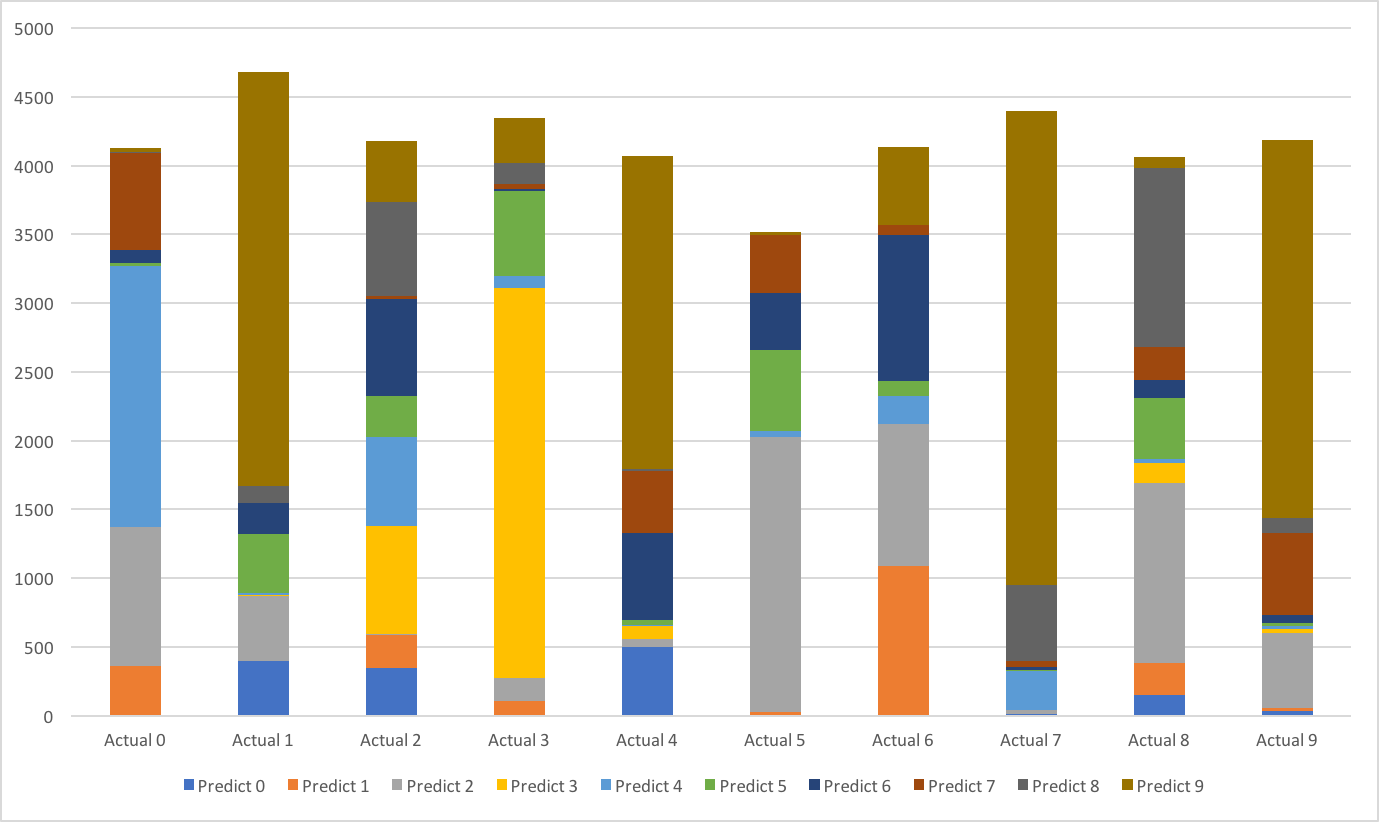
\includegraphics[width=1\textwidth]{images/mnist_test_result}
\caption{Mnist init.caffemodel test result}
\label{fig:samplepagoda}
\end{figure}

Because of Unsupervised Classification don't know what classes actually are. They just grouping the images, which they think there's the same into one class. So, we've to figure what these classes are.\newline
As the result above, we can easy to found some thing incorrect here: this model predicts 9 with very high percent in many classes: 1, 4, 7 and 9. \newline
The result scattered in different classes, so, we unable to know exactly what class actually are.

\subsubsection{Found the correct way to achieve the result}
After rereading the source code, carefully. I found that they were using KMeans Cluster to try to predict the closest cluster each sample in the test image belongs to.\newline
The most important part is:
\begin{lstlisting}
if (Y_pred != Y_pred_last).sum() < 0.001*N:
    print acc_list
    return acc, nmi
\end{lstlisting}
This is the terminal, the application achive the goal when the current predict (Y\_pred) is not different with the last predict. The value 0.001*N is threshold.\newline
So, at this time, we already have list of predicted images (in binary)

\subsubsection{Convert binary images into displayable images}
Because of the images used in the application is stored in binary \& read directly into memory. So, to be able to get the classified result, we've to convert image stored in memory (RAM) to the displayable image file. 

\begin{lstlisting}
def dispSingleImg(X, n, fname=None):
    h = X.shape[1]
    w = X.shape[2]
    c = X.shape[3]
    buff = np.zeros((h, w, c), dtype=np.uint8)

    buff[0:h, 0:w, :] = X[n]

    if fname is None:
        cv2.imshow('a', buff)
        cv2.waitKey(0)
    else:
        cv2.imwrite(fname, buff)
\end{lstlisting}
\begin{description}
\item[X:] array of image dataset
\item[n:] index of image
\item[fname:] destination to save
\end{description}

\subsubsection{Classify image dataset into X classes}
This feature put the images from dataset, which has the same class into one folder. This helps us to easy to verify the classified result

\begin{lstlisting}
def classify_dataset(predicts, imgs, db):
    classes_dir = "classes_" + db
    if not os.path.isdir(classes_dir):
        os.makedirs(classes_dir)
    for idex, pred in enumerate(predicts):
        tmp_dir = os.path.join(classes_dir, str(pred))
        if not os.path.isdir(tmp_dir):
            os.makedirs(tmp_dir)
        dispSingleImg(imgs, idex, os.path.join(tmp_dir, str(idex) + ".jpg"))
\end{lstlisting}
We call this function when the application predict done
\begin{lstlisting}
if (Y_pred != Y_pred_last).sum() < 0.001*N:
     classify_dataset(Y_pred, img, db)
     print acc_list
     return acc, nmi
\end{lstlisting}

\subsubsection{Generate the test summary result}

Because with mnist dataset, we already have the correct label of each image. So, to be able to summary the result, we add the following function to compare between predict \& actual result:

\begin{lstlisting}
def show_result(predicts, actuals):
    summary = {}
    for idx, value in enumerate(actuals):
        actual = str(value)
        predict = str(predicts[idx])
        if actual in summary:
            if predict in summary[actual]:
                summary[actual][predict] += 1
            else:
                summary[actual][predict] = 1
        else:
            summary[actual] = {}
    print summary
\end{lstlisting}
And call this function when the application predict done
\begin{lstlisting}
if (Y_pred != Y_pred_last).sum() < 0.001*N:
     classify_dataset(Y_pred, img, db)
     show_result(Y_pred, Y)
     print acc_list
     return acc, nmi
\end{lstlisting}

\subsubsection{Acquire and analytics the test result}
After run this network model with the \textbf{init.caffemodel}, we acquire the result describe as the following table:
\begin{table}[H]
\begin{center}
\begin{tabular}{| c | c | c | c | c | c | c | c | c | c | c |}
\hline
 & Predict 0 & 1 & 2 & 3 & 4 & 5 & 6 & 7 & 8 & 9\\
\hline
Actual 0 & 17 & 35 & 53 & 15 & 1 & 141 & 6629 & 1 & 4 & 6\\
\hline
1 & 7658 & 14 & 16 & 8 & 153 & 3 & 1 & 9 & 2 & 3\\
\hline
2 & 278 & 15 & 20 & 229 & 6094 & 42 & 73 & 29 & 112 & 87\\
\hline
3 & 108 & 128 & 13 & 178 & 171 & 6 & 12 & 23 & 67 & 6434\\
\hline
4 & 65 & 8 & 3060 & 8 & 7 & 58 & 3 & 3612 & 4 & 0\\
\hline
5 & 60 & 4968 & 41 & 133 & 6 & 54 & 7 & 37 & 13 & 899\\
\hline
6 & 233 & 268 & 2 & 37 & 14 & 6124 & 187 & 9 & 0 & 1\\
\hline
7 & 251 & 16 & 336 & 17 & 103 & 1 & 22 & 317 & 6226 & 3\\
\hline
8 & 167 & 142 & 62 & 5922 & 32 & 36 & 73 & 72 & 23 & 295\\
\hline
9 & 80 & 12 & 3624 & 60 & 5 & 16 & 47 & 2910 & 97 & 106\\

\hline
\end{tabular}
\caption {Mnist init.caffemodel test result}
\end{center}
\end{table}

\begin{figure}[H]
\centering
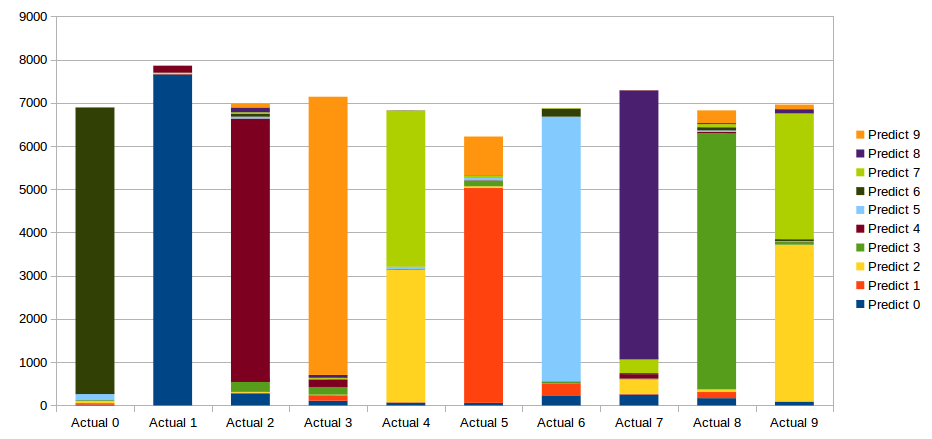
\includegraphics[width=1\textwidth]{images/mnist_test_result_2}
\caption{Mnist init.caffemodel test result v2}
\label{fig:samplepagoda}
\end{figure}

As the result above, we can easy to figure out that almost it can predict the images belong to which classes in high performance. Although it has a little confuse when predicting 2 and 7 but we can understand because of this two digit is similar.

Now we know how to receive the result of this implement source code. However, because of Mnist dataset is too simple. It just contains images, which has 28x28 pixel and only black \& white colors while our image Dataset has both bigger and true color. So, we need to try with the more complex Dataset. 

In the test Datasets they provide us has STL dataset, which closest with our Dataset (96 x 96 pixel, true color). We're going to try with this Dataset before try with we own dataset.

\subsection{Trying to run the implement code with STL dataset}
The application failure when execute \textbf{make\_stl\_data.py} python file to create STL LevelDB because of the "features.pyx" file is not delivery with the source code. 
I found that the author mention to the features.pyx at \href{https://github.com/cvondrick/pyvision/blob/master/vision/features.pyx}{https://github.com/cvondrick/pyvision/blob/master/vision/features.pyx}. However, when I test this file, I got another error
\begin{verbatim}
Type Error: "int" object is not iterable
\end{verbatim}
As the author say "It's been too long and I almost forgot about it, sorry. But you can try to refer to stackoverflow. I believe you can find your answer" (https://github.com/piiswrong/dec/issues/1). So, after some debug \& research, I found that the problem caused by the parameter of \textbf{function hog} in \textbf{feature.pyx} is an image object. But we provided an numpy object. So, I fixed it by replaced the following line in \textbf{features.pyx}
\begin{verbatim}
line 48. 		with, height = im.size
\end{verbatim}
by the following line:
\begin{verbatim}
line 48. 		with, height = im.shape[:2]
\end{verbatim}
Finally, it works. The accuracy result is 35.7\% (35.9\% in the paper).
\subsection{Preparing we own image dataset}
Below is the code we using to generate \& save data into LevelDB:
\begin{lstlisting}
import sys
import os
import Image
import numpy as np
import cv2
import cv
from joblib import Parallel, delayed
import features
import dec

def load_data(images_dir):
    ims = [read(os.path.join(images_dir, filename)) for filename in os.listdir(images_dir)]
    X = np.array(ims, dtype='uint8')
    n_jobs = 10
    cmap_size = (6, 10)
    N = X.shape[0]

    H = np.asarray(Parallel(n_jobs=n_jobs)(delayed(features.hog)(X[i]) for i in xrange(N)))

    H = H.reshape((H.shape[0], H.size / N))

    X_small = np.asarray(Parallel(n_jobs=n_jobs)(delayed(cv2.resize)(X[i], cmap_size) for i in xrange(N)))
    crcb = np.asarray(Parallel(n_jobs=n_jobs)(delayed(cv2.cvtColor)(X_small[i], cv.CV_RGB2YCrCb) for i in xrange(N)))
    crcb = crcb[:, :, :, 1:]
    crcb = crcb.reshape((crcb.shape[0], crcb.size / N))

    feature = np.concatenate(((H - 0.2) * 10.0, (crcb - 128.0) / 10.0), axis=1)
    print feature.shape

    return feature, X[:, :, :, [2, 1, 0]]


def load_label(images_dir, classes, determine):
    return np.array([classes.index(filename.split(determine)[0]) for filename in os.listdir(images_dir)], dtype='uint8')


def load_named_label(images_dir):
    return np.array([filename for filename in os.listdir(images_dir)], dtype='str')

if __name__ == '__main__':
    classes = ["heritage", "being", "scenery", "other"]
    images_dir = sys.argv[1]
    read = lambda imname: np.asarray(Image.open(imname).convert("RGB"))
    if os.path.isdir(images_dir):
        X_train, img_train = load_data(images_dir)
        Y = load_label(images_dir, classes, "_")
        labeled = load_named_label(images_dir)
        p = np.random.permutation(X_train.shape[0])
        X_total = X_train[p]
        Y_total = Y[p]
        labeled_total = labeled[p]
        np.save("custom_named_label", labeled_total)
        img_total = img_train[p]
        dec.write_db(X_total, Y_total, 'custom_total')
        dec.write_db(img_total, Y_total, 'custom_img')
        N = X_total.shape[0] * 4 / 5
        dec.write_db(X_total[:N], Y_total[:N], 'custom_train')
        dec.write_db(X_total[N:], Y_total[N:], 'custom_test')
    else:
        raise Exception("Please specific image url")

\end{lstlisting}


\subsection{Train with our dataset}

After train with our dataset, we get accurency 68.74\%

\begin{figure}[H]
\centering
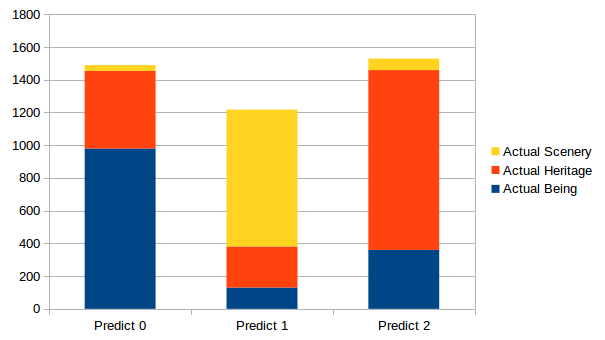
\includegraphics[width=1\textwidth]{images/unsupervised_large_dataset_result}
\caption{Unsupervised train result}
\end{figure}








\section{Supervised Deep Learning}
Supervised deep learning requires us to provide a training dataset, which includes a list of images labeled. However, our image dataset is not, and we can't classify the entire dataset by hand. So, we propose the following method, which includes three steps:
\begin{itemize}
\item Train a Convolution Neural Network (CNN) model with a small dataset based on the original dataset, which labeled by hand.
\item Use the CNN model trained above to classify the entire original dataset
\item Review \& Train a CNN model with the original dataset.
\end{itemize}

\subsection{Train a CNN model with a test dataset}

\subsubsection{Preparing test dataset based on original dataset}
We created this dataset by random 1000 images from the original dataset and classify them by hand into four classes: 
\begin{itemize}
\item Heritage
\item Beings
\item Scenery
\item Other
\end{itemize}
Below is the summary of each class in our dataset:

\begin{table}[H]
\begin{center}
\begin{tabular}{| c | c | c | c | c | c | c | c | c | c | c |}
\hline
 & Being & Heritage & Scenery & Other\\
\hline
count & 209 & 389 & 139 & 263\\
\hline
\end{tabular}
\caption {Test dataset summary}
\end{center}
\end{table}
Because in our dataset contain a lot of images, which have different resolution. So, we've to resize them all to the smallest resolution. The following script mainly to find \& resize all images 
\begin{lstlisting}
def get_lowest_resolution(image_dir):
    min_width, min_height = 9999, 9999
    for root, dirs, files in os.walk(images_dir):
        for f in files:
            image = os.path.join(root, f)
            width, height = Image.open(image).size
            min_width = lower(min_width, width)
            min_height = lower(min_height, height)
    return min_width, min_height


def lower(first, last):
    if first < last:
        return first
    return last

if __name__ == '__main__':
    images_dir = sys.argv[1]
    if os.path.isdir(images_dir):
        images_dir = os.path.abspath(images_dir)
        w, h = get_lowest_resolution(images_dir)
        for root, dirs, files in os.walk(images_dir):
            for f in files:
                image = os.path.join(root, f)
                print image
                im = Image.open(image).resize((w, h), Image.BICUBIC)
                im.save(image)

    else:
        raise Exception("Please specific image url")
\end{lstlisting}

\subsubsection{The caffe model for this CNN}
Our model is reuse from \href{https://github.com/BVLC/caffe/tree/master/models/bvlc\_reference\_caffenet}{bvlc\_reference\_caffenet} model, which is a replication of AlexNet with a few modifications. The original bvlc reference caffenet was designed for a classification problem with 1000 classes. However, we just need to classify into 4 classes. So, we change num output of the last
InnerProduct layer from 1000 to 4.

\subsubsection{The slover definition}
Our model using Stochastic Gradient Descent solver method. We run our model with 4000 iterators, drop leaning rate every 500 iterators and take a snapshot every 500 iterators.
\begin{verbatim}
 net: "caffe_model/caffenet_train.prototxt"
 test_iter: 500
 test_interval: 500
 base_lr: 0.001
 lr_policy: "step"
 gamma: 0.1
 stepsize: 500
 display: 50
 max_iter: 4000
 momentum: 0.9
 weight_decay: 0.0005
 snapshot: 1000
 snapshot_prefix: "caffe_model/snapshot"
 solver_mode: GPU
\end{verbatim}

\subsubsection{Acquire and analytics the test result}

After train the model with the test dataset, we obtain the result with very high loss \& low accuracy

\begin{figure}[H]
\centering
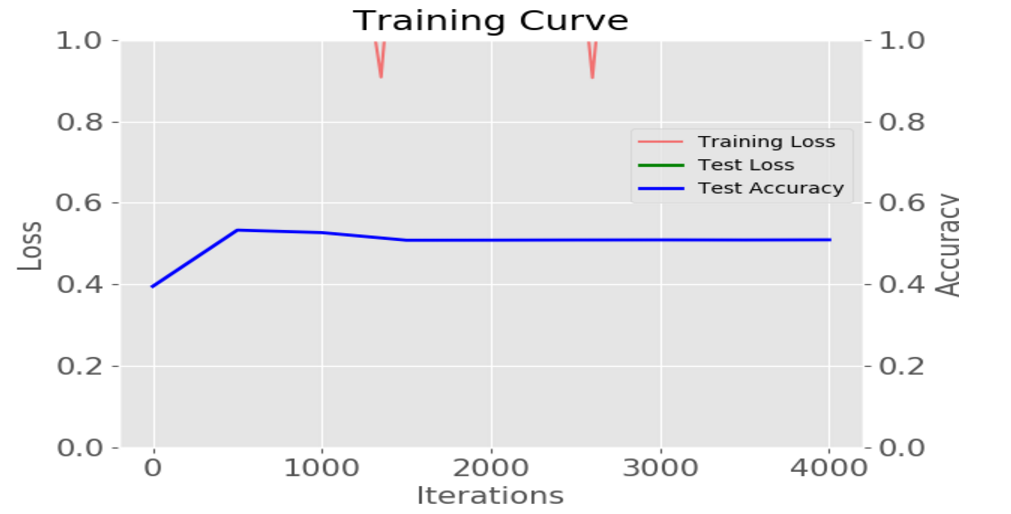
\includegraphics[width=1\textwidth]{images/train_first_time}
\caption{Train result}
\end{figure}
We tried to change the gamma parameter to 0.01, 0.001, 0.0001 but the result still the same. Trying to find the problem.

\subsubsection{Resolution problem}
Below is the summary of images dataset resolution. We assume that the image has resolution different no more than 10 pixels is the same solution.

\begin{figure}[H]
\centering
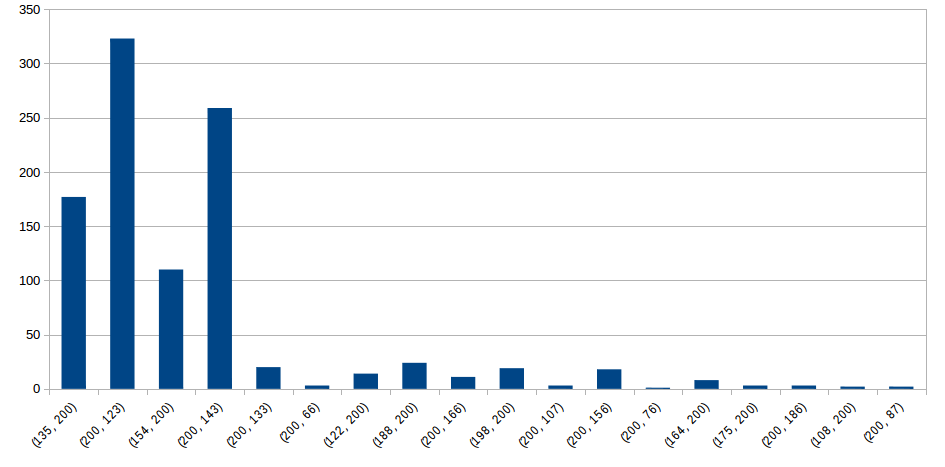
\includegraphics[width=1\textwidth]{images/resolution_summary}
\caption{Test Dataset resolution summary}
\end{figure}

As the result above, we have many different resolutions. We can't just resize all of them into the smallest. So, we keep the images, which have resolution (width, height) from (200, 120) to (200, 165) and discard the others.
Finally, we resize all images left to smallest resolution (200, 120)
Below is the summary of each class in our dataset:
\begin{table}[H]
\begin{center}
\begin{tabular}{| c | c | c | c | c | c | c | c | c | c | c |}
\hline
 & Being & Heritage & Scenery & Other\\
\hline
count & 140 & 160 & 127 & 189\\

\hline
\end{tabular}
\caption {Test dataset summary}
\end{center}
\end{table}

However, fixed this problem doesn't help us to reduce the loss when training the model. The lost still high, so we try to find another way to improve it.

\section{Train our model with only one class}
We have four classes includes being, heritage, scenery and other. We want to give a try to test and see how our model work when we train the model with just one class and ask whether this image belongs to this class or not.

\subsection{Train only being class}
With only being class, our dataset include: 
\begin{itemize}
\item 140 images - being class
\item 476 images - "all other" class
\end{itemize}

\subsubsection{Training progress}

\begin{figure}[H]
\centering
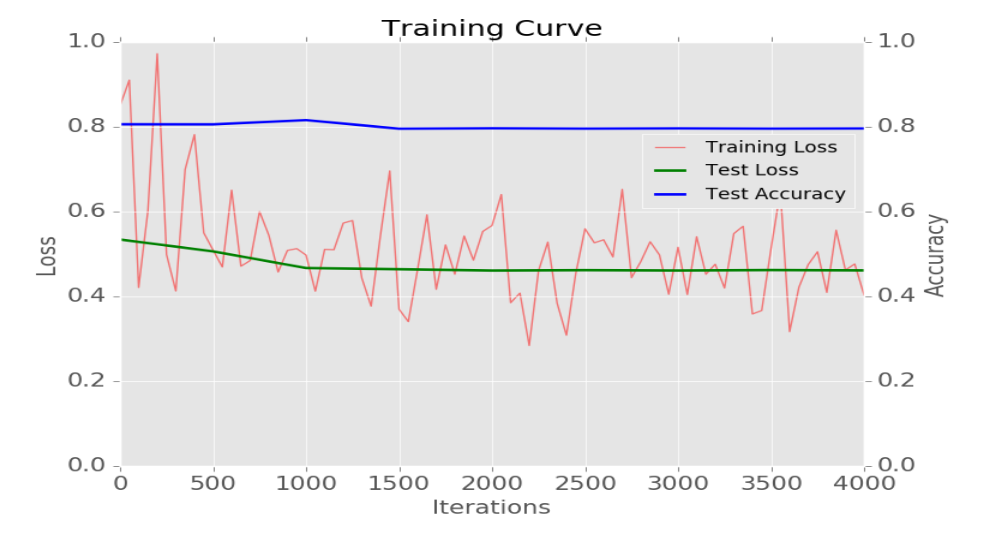
\includegraphics[width=1\textwidth]{images/train_only_being}
\caption{Being - training progress}
\end{figure}

\subsubsection{Training result}

\begin{figure}[H]
\centering
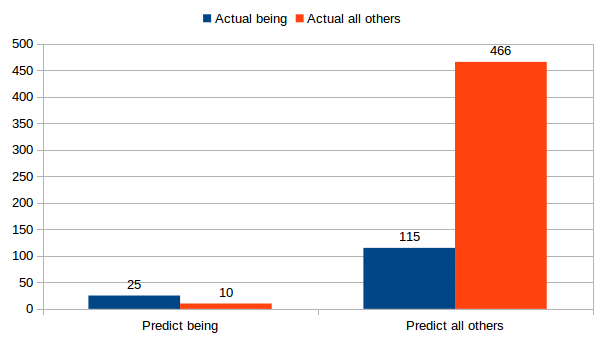
\includegraphics[width=1\textwidth]{images/being}
\caption{Being - training result}
\end{figure}


\subsection{Train only heritage class}
With only heritage class, our dataset include: 
\begin{itemize}
\item 160 images - heritage class
\item 456 images - "all other" class
\end{itemize}

\subsubsection{Training progress}

\begin{figure}[H]
\centering
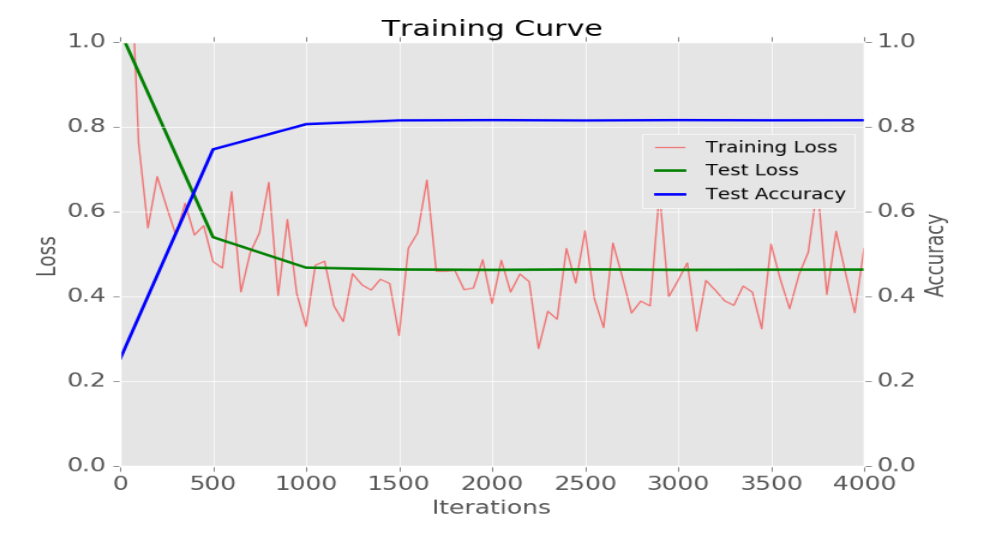
\includegraphics[width=1\textwidth]{images/train_only_heritage}
\caption{Heritage - training progress}
\end{figure}

\subsubsection{Training result}

\begin{figure}[H]
\centering
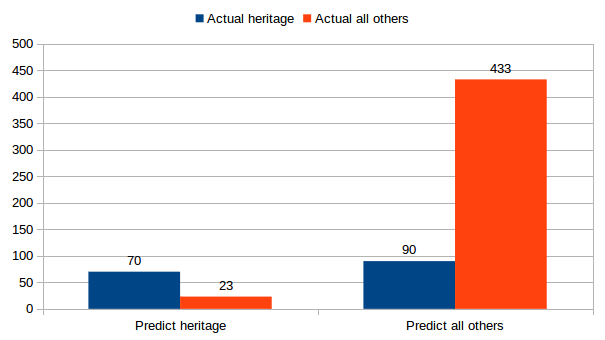
\includegraphics[width=1\textwidth]{images/heritage}
\caption{Heritage - training result}
\end{figure}

\subsection{Train only scenery class}
With only scenery class, our dataset include: 
\begin{itemize}
\item 127 images - scenery class
\item 489 images - "all other" class
\end{itemize}

\subsubsection{Training progress}

\begin{figure}[H]
\centering
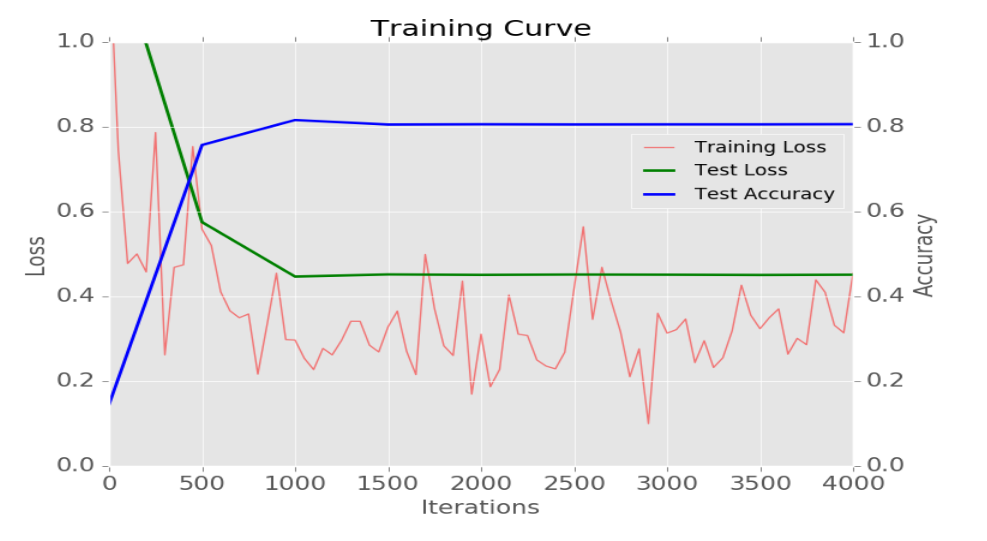
\includegraphics[width=1\textwidth]{images/train_only_scenery}
\caption{Scenery - training progress}
\end{figure}

\subsubsection{Training result}

\begin{figure}[H]
\centering
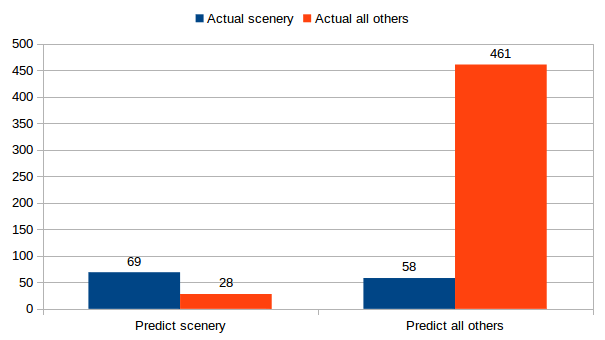
\includegraphics[width=1\textwidth]{images/scenery}
\caption{Scenery - training result}
\end{figure}

\subsection{Train only other class}
With only other class, our dataset include: 
\begin{itemize}
\item 189 images - other class
\item 427 images - "all other" class
\end{itemize}

\subsubsection{Training progress}

\begin{figure}[H]
\centering
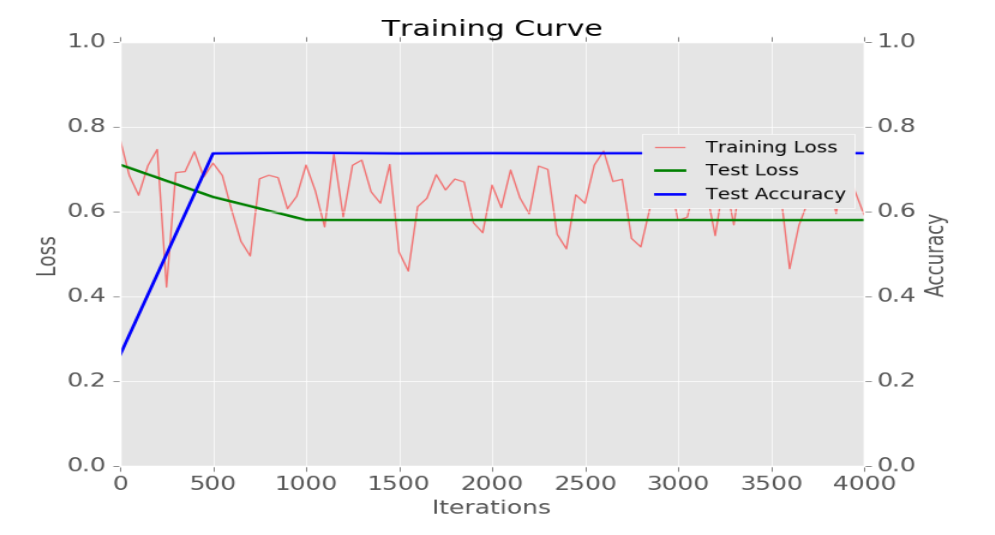
\includegraphics[width=1\textwidth]{images/train_only_other}
\caption{Other - training progress}
\end{figure}

\subsubsection{Training result}

\begin{figure}[H]
\centering
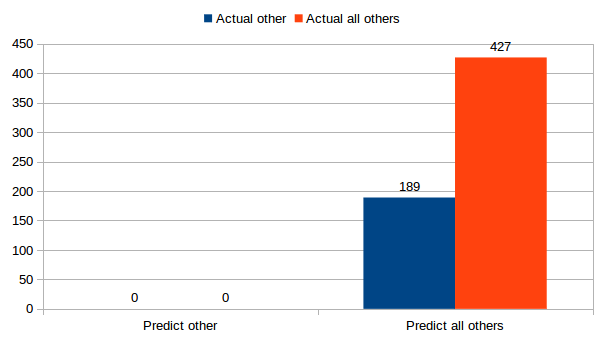
\includegraphics[width=1\textwidth]{images/other}
\caption{Other - training result}
\end{figure}

\section{Omit other class}
Because the other class, actually don't have any specialty. It just a place to keep all images, which don't belong to any other classes. So, It'll be a mistake if we continue to force our neural network to recognize it. 

\subsection{Train only being class}
With only being class, our dataset include: 
\begin{itemize}
\item 140 images - being class
\item 287 images - "all other" class
\end{itemize}

\subsubsection{Training progress}

\begin{figure}[H]
\centering
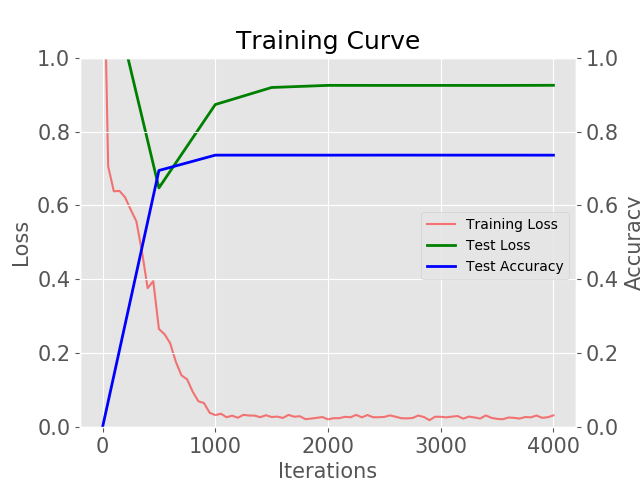
\includegraphics[width=1\textwidth]{images/train_omit_other_only_being}
\caption{Being - training progress}
\end{figure}

\subsubsection{Training result}

\begin{figure}[H]
\centering
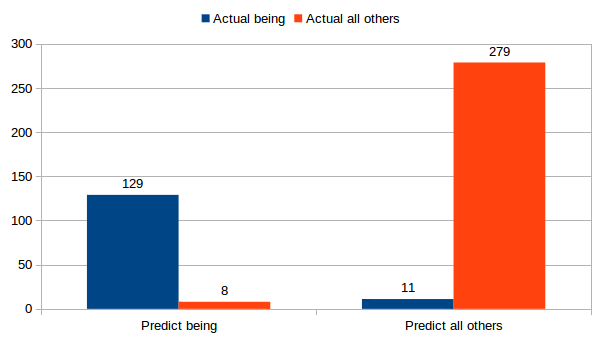
\includegraphics[width=1\textwidth]{images/omit_other_only_being}
\caption{Being - training result}
\end{figure}

This result seem to be good. But we're using the dataset, which used to train to test the model. So, it doesn't seem to the correct way to test. Therefore, we split our dataset into three small one. First (80\%) for training, second (10\%) for validate and lately, (10\%) for test.

\section{Test result}

After split our dataset, we have 43 images left for test.

\subsubsection{Training progress}

\begin{figure}[H]
\centering
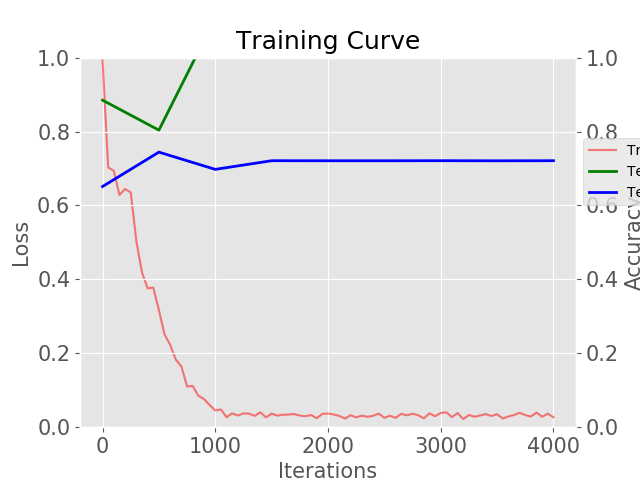
\includegraphics[width=1\textwidth]{images/only_being_43_images}
\caption{Being - training progress}
\end{figure}

\subsubsection{Training result}

\begin{figure}[H]
\centering
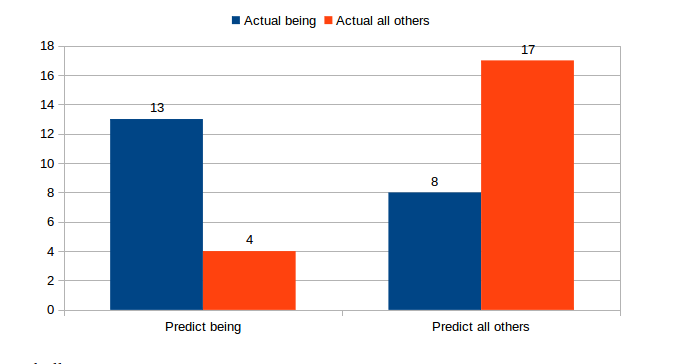
\includegraphics[width=1\textwidth]{images/test_43_image_result}
\caption{Being - training result}
\end{figure}

It's seem to we dont have enough images for both train \& test purpose. 

\section{Improve our dataset}

Because of lacking images so, we increase the size of our dataset by look back the original unlabeled images and get more images from them. We filter all images has too different size and then, we have 55477 images left. After that, we  look through all images and pick all images, which we sure it belong to the class that we are looking for. Finally, we have 4245 images include:
 
\begin{table}[H]
\begin{center}
\begin{tabular}{| c | c | c | c | c | c | c | c | c | c | c |}
\hline
 & Being & Heritage & Scenery\\
\hline
count & 1471 & 1832 & 942 \\
\hline
\end{tabular}
\caption {Test dataset summary}
\end{center}
\end{table}

\subsection{Training result}

We train our new dataset with 3 classes

\subsubsection{Training progress}

\begin{figure}[H]
\centering
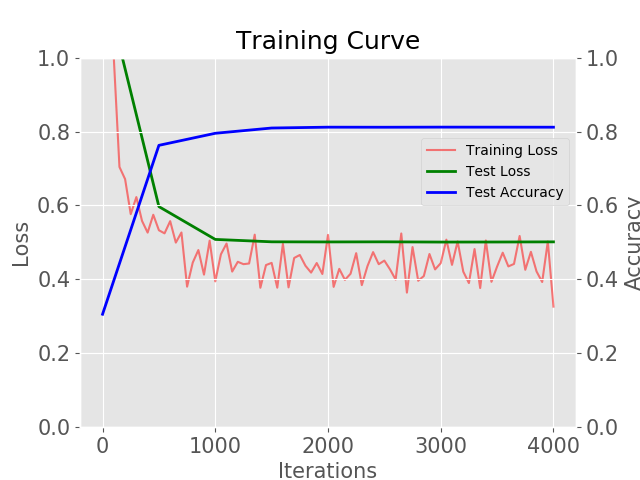
\includegraphics[width=1\textwidth]{images/70_10_20_train_large_dataset}
\caption{Train process}
\end{figure}

\begin{figure}[H]
\centering
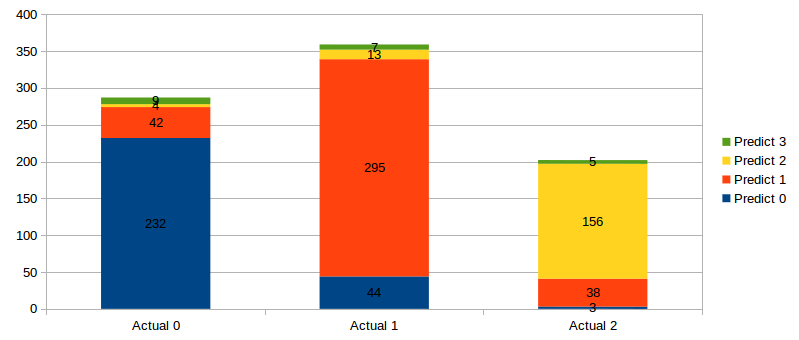
\includegraphics[width=1\textwidth]{images/70_10_20_result_large_dataset}
\caption{Test result}
\end{figure}


\subsection{Reduce Gamma from 0.1 to 0.01}

\subsubsection{Training progress}

\begin{figure}[H]
\centering
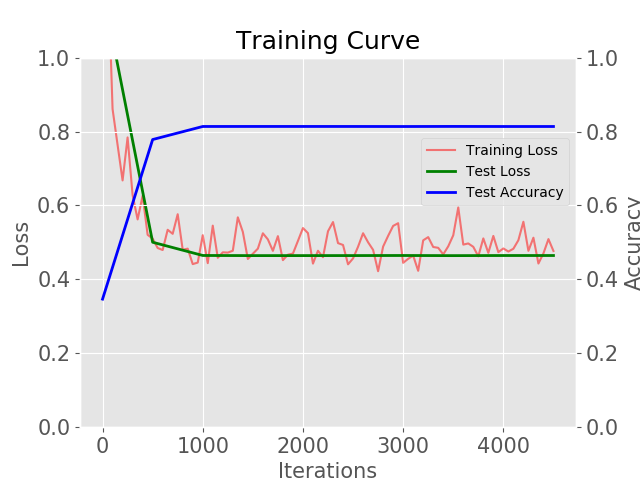
\includegraphics[width=1\textwidth]{images/train_large_dataset_gamma_0_01}
\caption{Train process}
\end{figure}

\begin{figure}[H]
\centering
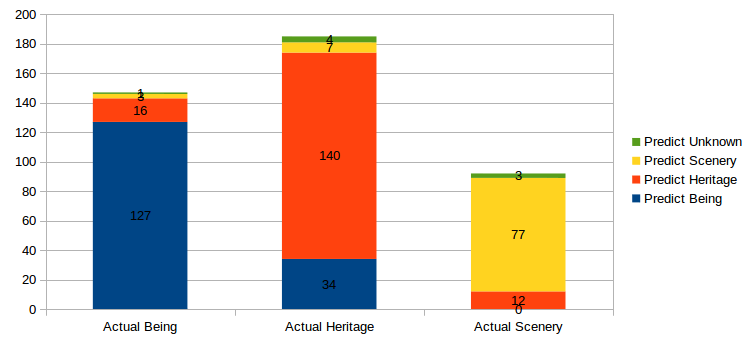
\includegraphics[width=1\textwidth]{images/test_large_dataset_gamma_0_01}
\caption{Test result}
\end{figure}

With 70\% train, 10\% validate and 20\% test

\subsubsection{Training progress}

\begin{figure}[H]
\centering
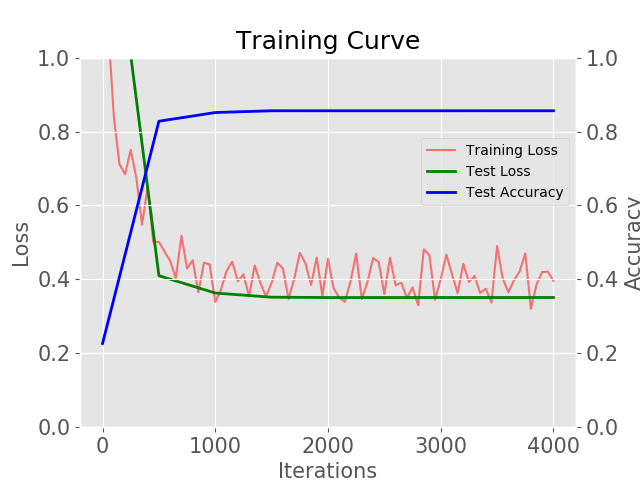
\includegraphics[width=1\textwidth]{images/train_large_dataset}
\caption{Train process}
\end{figure}

\begin{figure}[H]
\centering
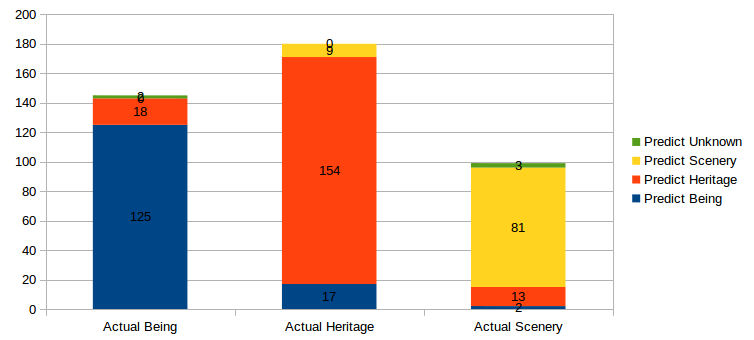
\includegraphics[width=1\textwidth]{images/result_large_dataset}
\caption{Test result}
\end{figure}

\subsection{Train with dataset come from unsupervised}
We using unsupervised to classify our images into 3 class. After that, we enter each class folder, remove all images, which not belong to current class. 

\subsubsection{Training progress}

\begin{figure}[H]
\centering
\includegraphics[width=1\textwidth]{images/train_dataset_from_unsupervised}
\caption{Train process}
\end{figure}

\begin{figure}[H]
\centering
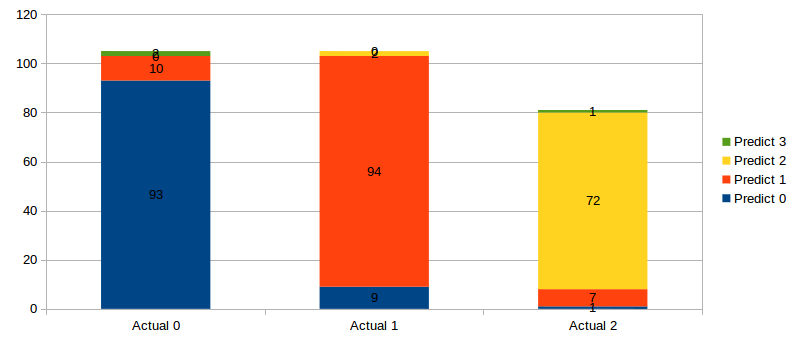
\includegraphics[width=1\textwidth]{images/result_dataset_from_unsupervised}
\caption{Test result}
\end{figure}

With 70\% train, 10\% validate and 20\% test

\begin{figure}[H]
\centering
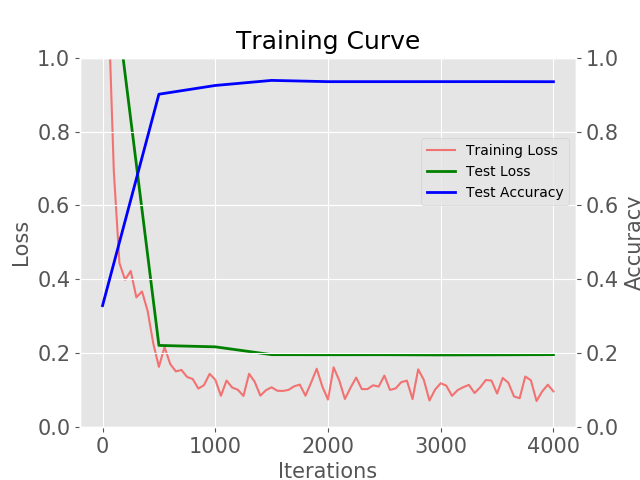
\includegraphics[width=1\textwidth]{images/70_10_20_train_dataset_from_unsupervised}
\caption{Train process}
\end{figure}

\begin{figure}[H]
\centering
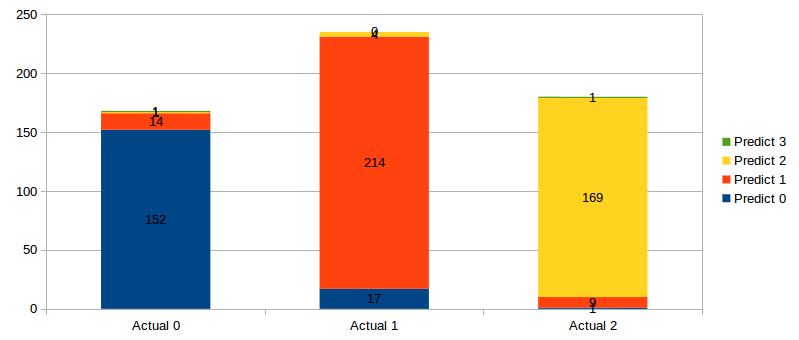
\includegraphics[width=1\textwidth]{images/70_10_20_result_dataset_from_unsupervised}
\caption{Test result}
\end{figure}

\bibliographystyle{ieeetr}
\bibliography{bibfile}
\end{document}